\documentclass{article}

% The package amsmath defines the environment equation*
\usepackage{amsmath}
% The package amssymb adds the macro \mathbb{...}
\usepackage{amssymb}
% The package amssymb adds the macro \degree
\usepackage{gensymb}
\usepackage{multicolrule}
\columnseprule=0.5pt
\usepackage{parskip}
% The package geometry allows to reduce the margin
\usepackage[
    a2paper,
    top=0.5cm,
    left=0.5cm,
    right=0.5cm,
    bottom=1.5cm
]{geometry}

\usepackage{titlesec}
\titleformat{\section}  % which section command to format
  {\fontsize{20}{20}\bfseries} % format for whole line
  {\thesection} % how to show number
  {1em} % space between number and text
  {} % formatting for just the text
  [] % formatting for after the text

\titleformat{\subsection}
  {\fontsize{18}{18}\bfseries} % format for whole line
  {\thesubsection} % how to show number
  {1em} % space between number and text
  {} % formatting for just the text
  [] % formatting for after the text

\usepackage{xcolor}
\usepackage{tikz}
\usetikzlibrary{arrows.meta}

% +-----------------------+
% |                       |
% | Símbolos customizados |
% |                       |
% +-----------------------+

\newsavebox \myequalbox
\sbox \myequalbox {%
    
\begin{tikzpicture}[scale=0.2, baseline]
        \coordinate (A) at (0,0);
        \coordinate (B) at (1.5,0);
        \coordinate (C) at (0,0.6);
        \coordinate (D) at (1.5,0.6);
        \draw[blue, line width = 1.5pt] (A) -- (B);
        \draw[blue, line width = 1.5pt] (C) -- (D);
    \end{tikzpicture}%
}

\newcommand\myequal{\mathrel{\vcenter{\hbox{\usebox\myequalbox}}}}

\newsavebox\myrightarrowbox
\sbox\myrightarrowbox{%
    
\begin{tikzpicture}[baseline=-0.7ex] % Adjusts vertical alignment
        \draw[red, line width = 1pt, -{Computer Modern Rightarrow[length=6pt, width=8pt]}] (0,0) -- (0.5,0);
    \end{tikzpicture}%
}
\newcommand\myrightarrow{\mathrel{\vcenter{\hbox{\usebox\myrightarrowbox}}}}

\newsavebox\myleftrightarrowbox
\sbox\myleftrightarrowbox{%
    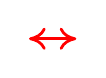
\begin{tikzpicture}[baseline=-0.7ex] % Adjusts vertical alignment
        \draw[red, line width = 1pt, {Computer Modern Rightarrow[length=6pt, width=8pt]}-{Computer Modern Rightarrow[length=6pt, width=8pt]}] (0,0) -- (0.6,0);
    \end{tikzpicture}%
}
\newcommand\myleftrightarrow{\mathrel{\vcenter{\hbox{\usebox\myleftrightarrowbox}}}}

\newsavebox\mylandbox
\sbox\mylandbox{%
    
\begin{tikzpicture}
        \draw[orange, line width = 1.5pt] (0,0) -- (0.15, 0.30) -- (0.3, 0);
    \end{tikzpicture}%
}

\newcommand\myland{\mathbin{\vcenter{\hbox{\usebox\mylandbox}}}}

% +--------------------------------------------------
% |
% | Inicio del documento
% |
% +--------------------------------------------------

\begin{document}
\fontsize{14pt}{14pt}\selectfont

\begin{multicols}{3}
\section{Identidades trigonométricas de ángulos simples}

Identidades recíprocas

\begin{itemize}
    \item $\sin\left(x\right) \cdot \csc\left(x\right) \myequal 1 \myrightarrow \csc\left(x\right) = \dfrac{1}{\sin\left(x\right)}$
    \item $\cos\left(x\right) \cdot \sec\left(x\right) \myequal 1 \myrightarrow \sec\left(x\right) = \dfrac{1}{\cos\left(x\right)}$
    \item $\tan\left(x\right) \cdot \cot\left(x\right) \myequal 1 \myrightarrow \cot\left(x\right) = \dfrac{1}{\tan\left(x\right)}$
\end{itemize}

Identidades por división o por cociente

\begin{itemize}
    \item $\tan\left(x\right) \myequal \dfrac{\sin\left(x\right)}{\cos\left(x\right)}$
    \item $\cot\left(x\right) \myequal \dfrac{\cos\left(x\right)}{\sin\left(x\right)}$
\end{itemize}

Identidades pitagóricas

\begin{itemize}
    \item $\sin^2\left(x\right) + \cos^2\left(x\right) \myequal 1$
    \item $\sec^2\left(x\right) \myequal 1 + \tan^2\left(x\right)$
    \item $\csc^2\left(x\right) \myequal 1 + \cot^2\left(x\right)$
\end{itemize}

Identidades auxiliares

\begin{itemize}
    \item $\left( \sin\left(x\right) \pm \cos\left(x\right) \right)^2 \myequal 1 \pm 2 \sin\left(x\right) \cos\left(x\right)$
    \item $\sin^4\left(x\right) + \cos^4\left(x\right) \myequal 1 - 2 \sin^2\left(x\right) \cos^2\left(x\right)$
    \item $\sin^6\left(x\right) + \cos^6\left(x\right) \myequal 1 - 3 \sin^2\left(x\right) \cos^2\left(x\right)$
    \item $\tan\left(x\right) + \cot\left(x\right) \myequal \sec\left(x\right) \csc\left(x\right)$
    \item $\sec^2 \left(x\right) + \csc^2 \left(x\right) \myequal \sec^2\left(x\right) \csc^2 \left(x\right)$
    \item $\sec\left(x\right) + \tan\left(x\right) \myequal \dfrac{1}{\sec\left(x\right) - \tan\left(x\right)}$
    \item $\csc\left(x\right) + \cot\left(x\right) \myequal \dfrac{1}{\csc\left(x\right) - \cot\left(x\right)}$
    \item $\left( 1 + \pm \sin\left(x\right) \pm \cos\left(x\right) \right)^2 \myequal 2 \left(1 \pm \sin\left(x\right)\right) \left(1 \pm \cos\left(x\right)\right)$
    \item $a \cdot \sin\left(x\right) + b \cos\left(x\right) = \sqrt{a^2 + b^2} \\ \myrightarrow  \sin\left(x\right) \myequal \dfrac{a}{\sqrt{a^2 + b^2}} \myland \cos\left(x\right) \myequal \dfrac{b}{\sqrt{a^2 + b^2}}$
\end{itemize}

\section{Identidades trigonométricas de ángulos compuestos}

Identidades de la suma y diferencia de dos ángulos

\begin{itemize}
    \item $\sin \left(x \pm y\right) \myequal \sin\left(x\right) \cos\left(y\right) \pm \cos\left(x\right) \sin\left(y\right)$
    \item $\cos \left(x \pm y\right) \myequal \cos\left(x\right) \cos\left(y\right) \mp \sin\left(x\right) \sin\left(y\right)$
    \item $\tan \left(x \pm y\right) \myequal \dfrac{\tan\left(x\right)\pm \tan\left(y\right)}{1 \mp \tan\left(x\right) \tan\left(y\right)}$
\end{itemize}

Identidades auxiliares de la suma y diferencia de dos ángulos

\begin{itemize}
     \item $\sin\left(x + y\right) \cdot \sin\left(x - y\right) \myequal \sin^2\left(x\right) - \sin^2\left(y\right)$
     \item $\cos\left(x + y\right) \cdot \cos\left(x - y\right) \myequal \cos^2\left(x\right) - \sin^2\left(y\right)$
     \item $\tan\left(\theta\right) \myequal \dfrac{b}{a} \myleftrightarrow a \cdot \sin\left(x\right) \pm b \cdot \cos\left(x\right) \myequal \sqrt{a^2 + b^2} \cdot \sin\left(x \pm \theta\right)$
     \item $\forall x \in \mathbb{R} : - \sqrt{a^2 + b^2} \leq a \cdot \sin\left(x\right) + b \cdot \cos\left(x\right) \leq \sqrt{a^2 + b^2}$
     \item $\tan\left(x \pm y\right) \myequal \tan\left(x\right) \pm \tan\left(y\right) \pm \tan\left(x\right) \tan\left(y\right) \tan\left(x \pm y\right)$
\end{itemize}

\subsection{Identidades para tres ángulos}

Si $\exists k \in \mathbb{Z} \colon x + y + z = k \pi$, entonces:

\begin{itemize}
    \item $\tan\left(x\right) + \tan\left(y\right) + \tan\left(z\right) \myequal \tan\left(x\right) \tan\left(y\right) \tan\left(z\right)$
    \item $\cot\left(x\right) \cot\left(y\right) + \cot\left(y\right) \cot\left(z\right) + \cot\left(z\right) \cot\left(x\right) \myequal 1$
\end{itemize}

Si $\exists k \in \mathbb{Z} \colon x + y + z = \displaystyle \dfrac{\left(2k+1\right) \pi}{2}$, entonces:

\begin{itemize}
    \item $\cot\left(x\right) + \cot\left(y\right) + \cot\left(z\right) \myequal \cot\left(x\right) \cot\left(y\right) \cot\left(z\right)$
    \item $\tan\left(x\right) \tan\left(y\right) + \tan\left(y\right) \tan\left(z\right) + \tan\left(z\right) \tan\left(x\right) \myequal 1$
\end{itemize}

\section{Identidades trigonométricas de múltiples ángulos}

\subsection{Identidades trigonométricas del ángulo doble}

\begin{itemize}
    \item $\sin\left(2x\right) \myequal 2 \sin\left(x\right) \cos\left(x\right)$
    \item $\cos\left(2x\right) \myequal \cos^2\left(x\right) - \sin^2\left(x\right)$
    \item $\tan\left(2x\right) \myequal \dfrac{2 \tan\left(x\right)}{1 - \tan^2\left(x\right)}$
    \item $\sin\left(2x\right) \myequal \dfrac{2 \tan\left(x\right)}{1 + \tan^2\left(x\right)}$
    \item $\cos\left(2x\right) \myequal \dfrac{1 - \tan^2\left(x\right)}{1 + \tan^2\left(x\right)}$
    \item $\cos\left(2x\right) \myequal 1 - 2 \sin^2\left(x\right) $
    \item $\cos\left(2x\right) \myequal 2 \cos^2\left(x\right) - 1$
\end{itemize}

Identidades de degradación

\begin{itemize}
    \item $2 \sin^2\left(x\right) \myequal 1 - \cos\left(2x\right)$
    \item $2 \cos^2\left(x\right) \myequal 1 + \cos\left(2x\right)$
    \item $8 \sin^4\left(x\right) \myequal 3 - 4 \cos\left(2x\right) + \cos\left(4x\right)$
    \item $8 \cos^4\left(x\right) \myequal 3 + 4 \cos\left(2x\right) + \cos\left(4x\right)$
    \item $\sin^4\left(x\right) + \cos^4\left(x\right) \myequal \dfrac{3}{4} + \dfrac{1}{4} \cos\left(4x\right)$
    \item $\sin^6\left(x\right) + \cos^6\left(x\right) \myequal \dfrac{5}{8} + \dfrac{3}{8} \cos\left(4x\right)$
\end{itemize}

Identidades auxiliares

\begin{itemize}
    \item $\left(\sin\left(x\right) \pm \cos\left(x\right)\right)^2 \myequal 1 \pm \sin\left(2x\right)$
    \item $\sqrt{1 \pm \sin\left(2x\right)} \myequal \left|\sin\left(x\right) \pm \cos\left(x\right)\right|$
    \item $\cot\left(x\right) + \tan\left(x\right) \myequal 2 \csc\left(2x\right)$
    \item $\cot\left(x\right) - \tan\left(x\right) \myequal 2 \cot\left(2x\right)$
    \item $\tan\left(2x\right) \cdot \cot\left(x\right) \myequal \sec\left(2x\right) + 1$
    \item $\tan\left(2x\right) \cdot \tan\left(x\right) \myequal \sec\left(2x\right) - 1$
\end{itemize}

\subsection{Identidades trigonométricas del ángulo mitad}

\begin{itemize}
    \item $\sin\left(\dfrac{x}{2}\right) \myequal \pm \sqrt{\dfrac{1 - \cos\left(x\right)}{2}}$
    \item $\cos\left(\dfrac{x}{2}\right) \myequal \pm \sqrt{\dfrac{1 + \cos\left(x\right)}{2}}$
    \item $\tan\left(\dfrac{x}{2}\right) \myequal \pm \sqrt{\dfrac{1 - \cos\left(x\right)}{1 + \cos\left(x\right)}}$
\end{itemize}

Identidades auxiliares
El signo de $\sin\left(\frac{x}{2}\right)$, $\cos\left(\frac{x}{2}\right)$ y $\tan\left(\frac{x}{2}\right)$ depende del cuadrante en el que se encuentra el lado final de $\frac{x}{2}$ y el signo de $\text{RT}\left(\frac{x}{2}\right)$ en ese cuadrante.


\begin{itemize}
    \item $\tan\left(\dfrac{x}{2}\right) \myequal \csc\left(x\right) - \cot\left(x\right)$
    \item $\cot\left(\dfrac{x}{2}\right) \myequal \csc\left(x\right) + \cot\left(x\right)$
\end{itemize}

\subsection{Identidades trigonométricas del ángulo triple}

\begin{itemize}
    \item $\sin\left(3x\right) \myequal 3 \sin\left(x\right) - 4 \sin^3\left(x\right)$
    \item $\cos\left(3x\right) \myequal 4 \cos^3\left(x\right) - 3 \cos\left(x\right)$
    \item $\tan\left(3x\right) \myequal \dfrac{3 \tan\left(x\right) - \tan^3\left(x\right)}{1 - 3 \tan^2\left(x\right)}$
\end{itemize}

Identidades de degradación

\begin{itemize}
    \item $4\sin^3\left(x\right) \myequal 3 \sin\left(x\right) - \sin\left(3x\right)$
    \item $4\cos^3\left(x\right) \myequal 3 \cos\left(x\right) + \cos\left(3x\right)$
\end{itemize}

Identidades auxiliares

\begin{itemize}
    \item $\dfrac{\sin\left(3x\right)}{\sin\left(x\right)} \myequal 2 \cos\left(2x\right) + 1$
    \item $\dfrac{\cos\left(3x\right)}{\cos\left(x\right)} \myequal 2 \cos\left(2x\right) - 1$
    \item $\dfrac{\tan\left(3x\right)}{\tan\left(x\right)} \myequal \dfrac{2 \cos\left(2x\right) + 1}{2 \cos\left(2x\right) - 1}$
    \item $\sin\left(3x\right) \myequal 4 \sin\left(x\right) \sin\left(60\degree - x\right) \sin\left(60 \degree + x\right)$
    \item $\cos\left(3x\right) \myequal 4 \cos\left(x\right) \cos\left(60\degree - x\right) \cos\left(60 \degree + x\right)$
    \item $\tan\left(3x\right) \myequal 4 \tan\left(x\right) \tan\left(60\degree - x\right) \tan\left(60 \degree + x\right)$
\end{itemize}

\end{multicols}
\end{document}
